\clearpage
\section{Altar Linens and Liturgical Books}
\PCDPlateHeader{Plate IV --- Altar and Vessel Linens}{Not to common scale}
\ifdefined\TriptychPrintEdition
\begin{center}
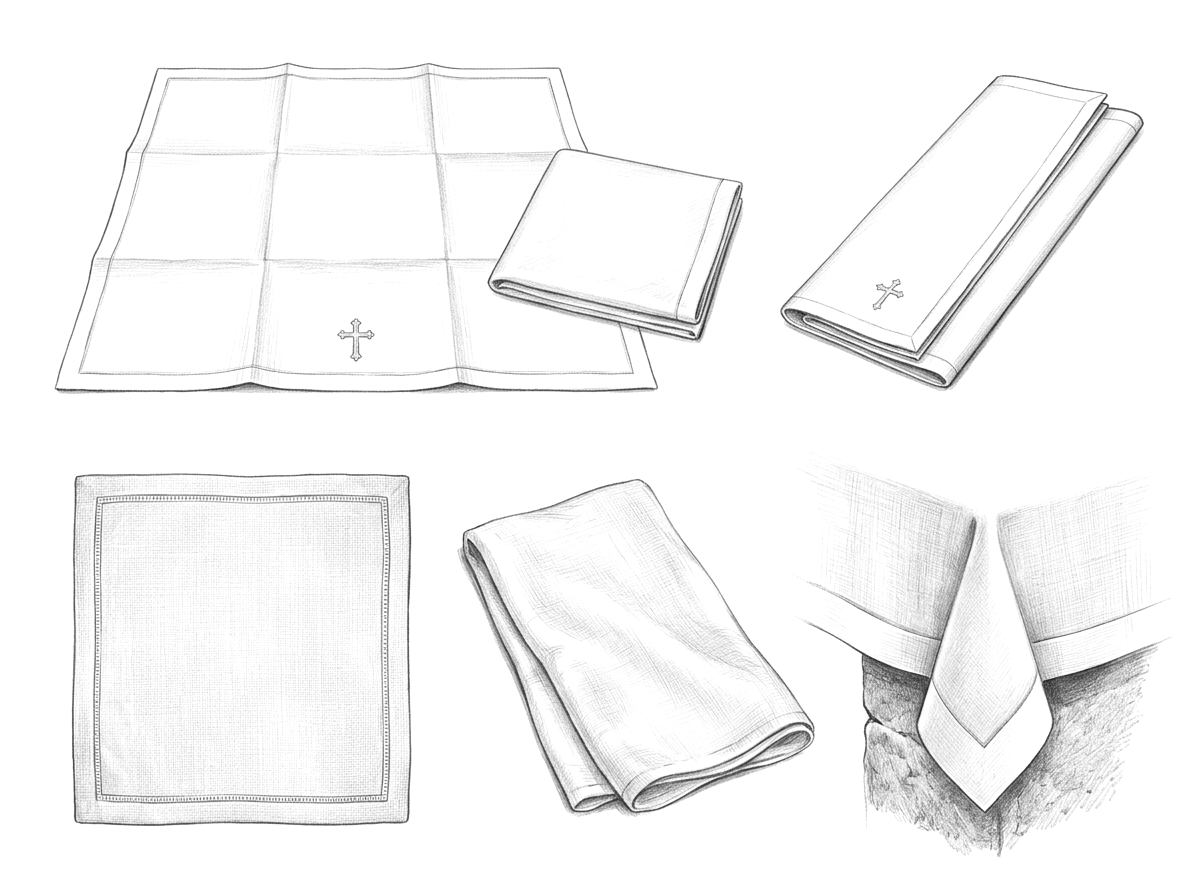
\includegraphics[width=0.92\linewidth,height=3.55in,keepaspectratio]{liturgy/roman-rite/postconciliar/2008-latin-2011-us-english/reference/roman-sanctuary-dictionary/shared/artwork/graphite/pc-art-04-white-linens.png}
\end{center}
\PCDPositionKey{Top left: unfolded square Corporal showing its three-by-three fold grid and front stitched cross, paired with a folded Corporal; top right: oblong Purificator folded lengthwise in thirds with stitched cross visible near the lower folded end; bottom left: stiffened square Pall; bottom center: folded Lavabo Towel; bottom right: hemmed corner of white Altar Cloth draped over the mensa.}
\else
\textbf{Visual Plate Summary (Plate IV --- Altar and Vessel Linens, Not to common scale):} Five-subject monochrome graphite textile study on pure white stock differentiating white altar linens by crease geometry and drape: top left, an unfolded square corporal creased into nine squares with a small stitched cross near the front center edge beside a folded square corporal; top right, an oblong purificator folded lengthwise in thirds with a small stitched cross visible near the lower folded end; bottom left, a rigid flat square linen pall; bottom center, a softly folded rectangular lavabo finger towel; bottom right, a hemmed corner of a white altar cloth hanging over a stone altar edge.

\textbf{Reading order and object placement:} Top left: unfolded square Corporal showing its three-by-three fold grid and front stitched cross, paired with a folded Corporal; top right: oblong Purificator folded lengthwise in thirds with stitched cross visible near the lower folded end; bottom left: stiffened square Pall; bottom center: folded Lavabo Towel; bottom right: hemmed corner of white Altar Cloth draped over the mensa.
\fi

\label{pc-obj-altar-cloth}
\PCDEntryHead{Altar Cloth}{Mappa}{required}{N15}
\PCDField{Also called}{Fair linen; Altar linen; \textit{Mappa altaris}; \textit{Mappae}; \textit{Tobalea}}
Verify before every Mass that at least one spotless, freshly pressed white linen altar cloth covers the mensa cleanly and matches the altar's proportions (GIRM 117, 304). Where your parish uses the United States adaptation permitting festive colored under-cloths beneath the white top cloth (US GIRM 304), align hems evenly with no wrinkled layers. Inspect regularly for wax drips or stains, and if the Precious Blood has touched the altar cloth, wash the affected area first by hand and pour the rinse water into the sacrarium or clean earth before ordinary laundering (GIRM 280; RS 120).

\PCDField{Plate position and norm}{Bottom right corner drape (Plate IV); dressing the altar (Plates I--II) (Universal Roman law)}
\PCDField{Placement and use}{Laid smoothly over the altar mensa before Mass so that at least one clean white cloth always covers the table of sacrifice (GIRM 117, 304). Any under-cloths---including festive colored under-cloths permitted in United States dioceses---lie neatly beneath the white uppermost cloth. Until the Preparation of the Gifts, the dressed mensa remains uncluttered, holding no cruets, stands, or loose papers (GIRM 306).}
\PCDField{United States norm}{In the Dioceses of the United States of America, the confirmed territorial adaptation at GIRM 304 permits additional altar cloths beneath or alongside the primary cloth to bear other colors of Christian honorific or festive significance, provided the uppermost cloth covering the mensa is always white.}
\PCDField{Prepared and handled by}{Prepares: Sacristan, Instituted acolyte, Altar server. Ministers in use: Bishop, Priest, Deacon.}
\PCDSafety{Never blot or wash a spill of the Precious Blood on the altar cloth yourself; notify the priest or deacon at once so the spot is washed with water and the ablution poured into the sacrarium (GIRM 280; RS 120). Guard the linen against candle flames and molten wax.}
\PCDField{Distinguish from}{Corporal, Lavabo Towel}
\PCDEntryRule

\label{pc-obj-corporal}
\PCDEntryHead{Corporal}{Corporale}{required}{N16}
\PCDField{Also called}{Altar corporal; \textit{Palla corporalis}}
Starch corporals lightly and press them crisply into nine equal squares folded inward---bottom over middle, top over middle, right over middle, left over middle---so the inner surface stays protected and the front cross aligns toward the celebrant when opened. Prepare one clean corporal on the credence table for Mass (GIRM 118c) and keep spare clean corporals ready for vessels awaiting post-Mass purification (GIRM 279) or Eucharistic Exposition. After Mass, strictly follow Redemptionis Sacramentum 120: soak and hand-rinse used corporals first in a dedicated basin and pour the first rinse water into the sacrarium or clean earth before ordinary washing and ironing. Note that while GIRM 118c praises the chalice veil, it does not list a stiff burse.

\PCDField{Plate position and norm}{Top left, shown unfolded in a 3x3 crease grid and folded beside it (Plate IV); beneath vessels (Plate X) (Universal Roman law)}
\PCDField{Placement and use}{Prepared neatly folded on the credence table (GIRM 118c), brought to the altar at the Preparation of the Gifts, and spread open at the center of the mensa by the deacon, instituted acolyte, or priest (GIRM 139, 178, 190). After Communion and vessel purification, the minister folds the sides carefully inward---enclosing the upper surface inside---so no microscopic particle of the Sacred Host can scatter (GIRM 183, 192). Unpurified vessels left on the altar or credence table after Mass likewise rest suitably covered on a corporal (GIRM 279).}
\PCDField{United States norm}{Universal Roman law requires a corporal beneath all Eucharistic vessels on the altar (GIRM 118c, 139, 306) and beneath unpurified vessels awaiting post-Mass purification (GIRM 279; USCCB Norms for Holy Communion under Both Kinds 53). While GIRM 118c commends the optional chalice veil, it does not mention the stiff burse, which remains purely a traditional accessory.}
\PCDField{Prepared and handled by}{Prepares: Sacristan, Deacon, Instituted acolyte, Altar server. Ministers in use: Bishop, Priest, Deacon, Instituted acolyte.}
\PCDSafety{A used corporal may hold fine particles of the Sacred Host. Never shake it out or wash it directly in an ordinary sink; first soak and hand-rinse it in a dedicated basin and pour that first rinse water into the sacrarium or directly into clean earth before ordinary laundering (RS 120).}
\PCDField{Distinguish from}{Purificator, Pall, Lavabo Towel, Altar Cloth}
\PCDEntryRule

\label{pc-obj-purificator}
\PCDEntryHead{Purificator}{Purificatorium}{required}{N17}
\PCDField{Also called}{Chalice cloth}
Prepare one clean, unstarched absorbent linen purificator folded lengthwise in thirds for the principal chalice and one fresh purificator for each additional Communion chalice whenever Communion under both kinds is celebrated (GIRM 118c, 286). Skip heavy starch so the linen absorbs cleanly along the chalice rim. After Mass, collect all used purificators strictly apart from lavabo towels, soak and hand-rinse them first in a dedicated basin, and pour the first rinse water into the sacrarium or directly into clean earth before ordinary washing and ironing (RS 120).

\PCDField{Plate position and norm}{Top right, folded lengthwise in thirds with stitched cross visible near the lower folded end (Plate IV); beside Communion cups (Plate X) (Universal Roman law)}
\PCDField{Placement and use}{Prepared on the credence table draped across the principal chalice---and paired one-to-one beside every additional Communion chalice whenever Communion is distributed under both kinds (GIRM 118c, 286). During Communion, the minister of the chalice wipes both sides of the rim with a clean fold after each communicant; after Communion, the priest, deacon, or instituted acolyte dries the purified sacred vessels with it at the altar or credence table (GIRM 279, 306).}
\PCDField{United States norm}{Under GIRM 286 and the 2011 USCCB Norms for Holy Communion under Both Kinds (nos. 43, 53), one clean purificator accompanies every Communion chalice to wipe the rim after each communicant, and post-Communion vessel purification using the purificator belongs exclusively to the priest, deacon, or instituted acolyte.}
\PCDField{Prepared and handled by}{Prepares: Sacristan, Deacon, Instituted acolyte, Altar server. Ministers in use: Bishop, Priest, Deacon, Instituted acolyte, Extraordinary minister of Holy Communion.}
\PCDSafety{Used purificators hold traces of the Precious Blood. Never wash a used purificator in an ordinary sink or mix it into regular laundry; soak and hand-rinse it first in a dedicated basin and pour that first rinse water into the sacrarium or directly into clean earth before ordinary laundering (RS 120).}
\PCDField{Distinguish from}{Lavabo Towel, Corporal, Pall}
\PCDEntryRule

\label{pc-obj-pall}
\PCDEntryHead{Pall}{Palla}{optional}{N18}
\PCDField{Also called}{Chalice pall; \textit{Palla calicis}}
Keep clean, unwarped palls ready on the credence table whenever appropriate (GIRM 118c)---especially during summer months, open-window ventilation, or outdoor celebrations where dust or insects might fall into the chalice. Inspect the underside before every Mass for stains; remove any plastic or card insert before washing, and whenever the linen has contacted the Precious Blood, perform the sacrarium first-rinse mandated by Redemptionis Sacramentum 120 before regular laundering.

\PCDField{Plate position and norm}{Bottom left, stiffened square (Plate IV) (Universal Roman law)}
\PCDField{Placement and use}{Prepared on the credence table atop the chalice and paten whenever appropriate---explicitly qualified as optional (pro opportunitate, ``if appropriate'') in GIRM 118c---and permitted on the altar mensa during the Liturgy of the Eucharist (GIRM 139, 306). The priest or deacon lifts it before pouring, consecrating, or drinking, and replaces it whenever dust, drafts, or insects threaten an open chalice, especially in warm seasons or outdoor Masses.}
\PCDField{Prepared and handled by}{Prepares: Sacristan, Deacon, Instituted acolyte, Altar server. Ministers in use: Bishop, Priest, Deacon.}
\PCDSafety{Remove any rigid insert before washing a slipcover pall; if drops of the Precious Blood ever touch the linen underside, soak and hand-rinse the linen first into the sacrarium or clean earth before ordinary laundering (RS 120).}
\PCDField{Distinguish from}{Corporal, Purificator}
\PCDEntryRule

\label{pc-obj-lavabo-towel}
\PCDEntryHead{Lavabo Towel}{Manutergium}{required}{N19}
\PCDField{Also called}{Finger towel; Hand towel; \textit{Tersorium}}
Set a fresh, dry, absorbent white hand towel beside the filled lavabo pitcher and empty finger basin on the credence table before each Mass (GIRM 118c), replacing damp towels between consecutive celebrations. Because the lavabo towel touches only clean washing water and never contacts the Sacred Species, launder it with ordinary church linens and store it in a clearly separate drawer from corporals and purificators.

\PCDField{Plate position and norm}{Bottom center, softly folded rectangular cloth (Plate IV); paired with lavabo pitcher and basin (Plate VI) (Universal Roman law)}
\PCDField{Placement and use}{Prepared on the credence table beside the lavabo pitcher and basin (GIRM 118c appoints whatever is needed for the washing of hands). At the Preparation of the Gifts---immediately after the offerings are placed on the altar or after the incensation---an altar server or instituted acolyte pours water over the priest's hands at the side of the altar and presents the unfolded towel while the priest prays quietly for interior cleansing (GIRM 76, 145, 190).}
\PCDField{Prepared and handled by}{Prepares: Sacristan, Instituted acolyte, Altar server. Ministers in use: Bishop, Priest.}
\PCDSafety{Keep plain lavabo towels strictly separate from sacred purificators in both the sacristy and credence setup so the two are never interchanged. Hold the pitcher and basin level so water does not splash onto the altar cloth or sanctuary steps.}
\PCDField{Distinguish from}{Purificator, Corporal}
\PCDEntryRule

\clearpage
\PCDPlateHeader{Plate V --- Liturgical Books and Stands}{Relative proportions shown}
\ifdefined\TriptychPrintEdition
\begin{center}
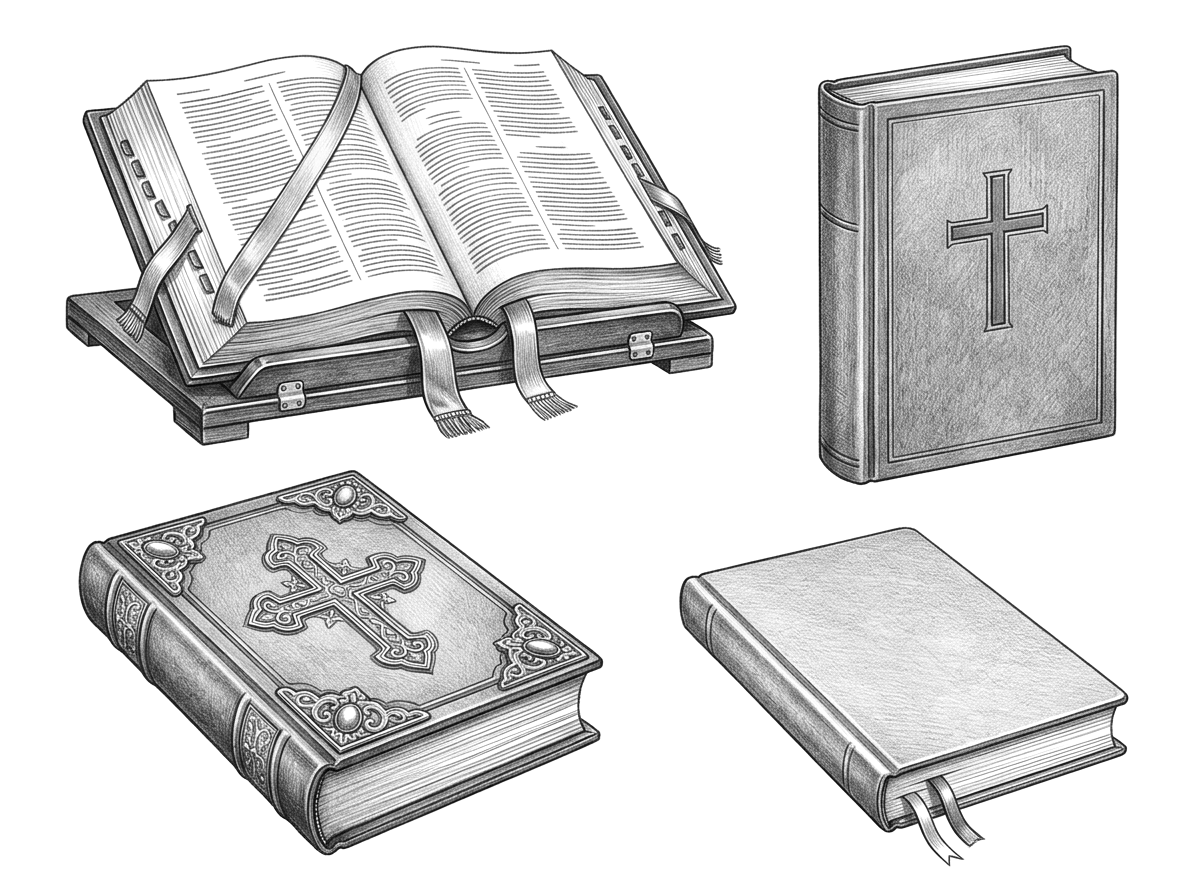
\includegraphics[width=0.92\linewidth,height=3.55in,keepaspectratio]{liturgy/roman-rite/postconciliar/2008-latin-2011-us-english/reference/roman-sanctuary-dictionary/shared/artwork/graphite/pc-art-05-liturgical-books.png}
\end{center}
\PCDPositionKey{Top left: thick Roman Missal open with side tabs and ribbon markers on a low angled Missal Stand; top right: tall closed Lectionary for Mass; bottom left: ornate bound Book of the Gospels (Evangeliary) with metal corner bosses and embossed cross; bottom right: slimmer Book of the Chair (Excerpts from the Roman Missal).}
\else
\textbf{Visual Plate Summary (Plate V --- Liturgical Books and Stands, Relative proportions shown):} Four-book monochrome graphite comparison showing relative scale and binding dignity: top left, a thick altar Roman Missal open flat with ribbon markers and edge tabs on a low angled wooden stand; top right, a tall closed hardcover Lectionary marked with a plain cover cross; bottom left, a heavily ornamented Book of the Gospels with sculpted metal corner bosses and central embossed cross; bottom right, a slimmer handheld Book of the Chair with two ribbon markers.

\textbf{Reading order and object placement:} Top left: thick Roman Missal open with side tabs and ribbon markers on a low angled Missal Stand; top right: tall closed Lectionary for Mass; bottom left: ornate bound Book of the Gospels (Evangeliary) with metal corner bosses and embossed cross; bottom right: slimmer Book of the Chair (Excerpts from the Roman Missal).
\fi

\label{pc-obj-roman-missal}
\PCDEntryHead{Roman Missal}{Missale Romanum}{required}{N20}
\PCDField{Also called}{Altar Missal; Sacramentary (1974--2011 U.S. usage); \textit{Missale}}
Always prepare the complete, officially approved Roman Missal---never loose sheets or disposable binders---setting side tabs and ribbon markers cleanly for the Collect, Prayer over the Offerings, proper Preface, appointed Eucharistic Prayer, Prayer after Communion, and any Solemn Blessing or Prayer over the People (GIRM 118a, 349, 389). Stage the Missal beside the presidential chair (or on the credence table whenever the Book of the Chair is used at the chair) so the altar mensa remains bare until the Preparation of the Gifts (GIRM 306).

\PCDField{Plate position and norm}{Top left, open with edge tabs and ribbons on a low stand (Plate V) (Universal Roman law)}
\PCDField{Placement and use}{Prepared beside the presidential chair before Mass (GIRM 118a, unless the Book of the Chair is used for chair prayers) and placed on the altar at the Preparation of the Gifts so the priest prays the Prayer over the Offerings, Preface, Eucharistic Prayer, and Communion rites directly from it (GIRM 139, 306). After the purification of vessels, it may return to the presidential chair for the Prayer after Communion and Solemn Blessing (GIRM 165--167, 306).}
\PCDField{United States norm}{In the Dioceses of the United States of America, the approved vernacular edition is The Roman Missal, Third Edition (USCCB, effective 27 November 2011), translating the 2002/2008 Latin third typical edition in its entirety (GIRM 389) and incorporating confirmed United States adaptations and the 2021 emendations.}
\PCDField{Prepared and handled by}{Prepares: Sacristan, Deacon, Instituted acolyte, Altar server. Ministers in use: Bishop, Priest.}
\PCDSafety{Support the heavy altar Missal evenly with both hands or braced cleanly against your upper chest---never by one cover---so the binding does not tear or slip. Never set loose announcements, bulletins, or unapproved sheets atop the Missal or on the altar mensa (GIRM 306).}
\PCDField{Distinguish from}{Book of the Chair, Lectionary for Mass, Book of the Gospels}
\PCDEntryRule

\label{pc-obj-lectionary}
\PCDEntryHead{Lectionary for Mass}{Lectionarium}{required}{N21}
\PCDField{Also called}{Lectionary; \textit{Ordo lectionum Missae}}
Confirm the exact volume and liturgical cycle before every Mass---Sunday Year A, B, or C; Weekday Year I or II; or Proper of Saints and Ritual Masses---mark the passages with the ribbon, and set the Lectionary open on the ambo before the entrance procession starts (GIRM 118b). Never substitute disposable paper booklets, loose sheets, or worn copies for the dignified ritual Lectionary at the ambo (GIRM 349; OLM 35--37).

\PCDField{Plate position and norm}{Top right, tall closed volume with cover cross (Plate V) (Universal Roman law)}
\PCDField{Placement and use}{Placed open to the day's readings on the stationary ambo before Mass begins (GIRM 118b). Instituted lectors and deputed readers proclaim the first and second readings from it at the ambo, and the deacon or priest proclaims the Gospel from it whenever a separate Book of the Gospels is not employed. Under universal Roman rubrics (GIRM 120d, 194), the Lectionary is never carried in the entrance procession---only the Book of the Gospels receives that ceremonial procession.}
\PCDField{United States norm}{In the Dioceses of the United States of America, Scripture readings at Mass are proclaimed from the approved Lectionary for Mass for Use in the Dioceses of the United States (Confraternity of Christian Doctrine), arranged according to the 1981 editio typica altera of the Ordo lectionum Missae; disposable booklets or parish missalettes never replace the ritual Lectionary on the ambo (GIRM 349; OLM 35--37).}
\PCDField{Prepared and handled by}{Prepares: Sacristan, Instituted lector, Altar server. Ministers in use: Bishop, Priest, Deacon, Instituted lector.}
\PCDSafety{Never carry the Lectionary in the entrance procession---GIRM 120d and 194 strictly reserve the entrance book procession to the Book of the Gospels. Never replace the ritual Lectionary on the ambo with disposable paper leaflets or pew missalettes (GIRM 349).}
\PCDField{Distinguish from}{Book of the Gospels, Roman Missal}
\PCDEntryRule

\label{pc-obj-book-of-the-gospels}
\PCDEntryHead{Book of the Gospels}{Evangeliarium}{provided}{N22}
\PCDField{Also called}{Evangeliary; Gospel Book; \textit{Liber Evangeliorum}}
Strongly commended by the Church (OLM 36), the Book of the Gospels should visibly surpass every other sanctuary volume in beauty and craftsmanship (GIRM 349). Before Mass, verify and ribbon-mark the appointed Gospel passage, check clasps or heavy metal covers so pages lie flat on the ambo without slipping, and place the closed volume ready for the deacon (or lector if no deacon serves) in the procession area---never pre-set on the ambo, since it enters in procession and rests on the altar until the Alleluia (GIRM 120d, 122, 306). After Mass, return it cleanly to its protective case or display stand.

\PCDField{Plate position and norm}{Bottom left, ornate metal-bossed cover (Plate V) (Universal Roman law)}
\PCDField{Placement and use}{Strongly commended for cathedrals and parishes (OLM 36). Carried slightly elevated in the entrance procession by the deacon---or, in the deacon's absence, by an instituted or deputed lector---and laid flat on the center of the altar, the sole book permitted upon the mensa from the beginning of Mass until the Gospel (GIRM 120d, 122, 172--173, 194, 306). At the Gospel Acclamation, the deacon (or priest, if no deacon serves) lifts it from the altar and carries it to the ambo accompanied by servers with lighted candles and incense; after three swings of incense (GIRM 277; executed as paired double swings in Roman ceremonial custom, Caeremoniale Episcoporum 92) and proclamation, the minister reverently kisses the book while praying quietly Per evangelica dicta (GIRM 134, 175).}
\PCDField{United States norm}{In the Dioceses of the United States of America, the approved Book of the Gospels contains the Sunday and feast-day Gospels in the Lectionary translation and is customarily bound in embossed metallic or richly ornamented covers honoring the dignity commended by GIRM 349 and OLM 36--37.}
\PCDField{Prepared and handled by}{Prepares: Sacristan, Deacon, Instituted lector. Ministers in use: Bishop, Priest, Deacon, Instituted lector.}
\PCDSafety{Never hand the Book of the Gospels to an altar server to carry in the entrance procession---GIRM 120d and 194 reserve that role strictly to the deacon or, in his absence, a lector. During the Gospel procession, candle-bearers hold flames well clear of the ornate cover and open pages.}
\PCDField{Distinguish from}{Lectionary for Mass, Roman Missal}
\PCDEntryRule

\label{pc-obj-book-of-the-chair}
\PCDEntryHead{Book of the Chair}{Excerpts from the Roman Missal (no Latin typical edition)}{territorial adaptation}{N23}
\PCDField{Also called}{Excerpts from the Roman Missal; Presidential Prayer Book}
Mark both ribbons in Excerpts from the Roman Missal before Mass for the day's Collect, Prayer after Communion, and any Solemn Blessing or Prayer over the People, setting it neatly beside the presidential chair (GIRM 118a). Always prepare the full Roman Missal separately on the credence table (marked for the Prayer over the Offerings, Preface, and Eucharistic Prayer) so the Liturgy of the Eucharist never lacks its complete altar book (GIRM 139, 306).

\PCDField{Plate position and norm}{Bottom right, slimmer handheld ceremonial volume (Plate V) (USCCB territorial adaptation)}
\PCDField{Placement and use}{Placed beside the presidential chair before Mass (fulfilling GIRM 118a) and held open by an altar server or set on a discreet chair stand for the Introductory Rites, Collect, concluding prayer of the Universal Prayer, Prayer after Communion, and Final Blessing. Because it omits the Prefaces and Eucharistic Prayers, it is never placed on the altar mensa in place of the complete Roman Missal (GIRM 139, 306).}
\PCDField{United States norm}{Officially titled Excerpts from the Roman Missal, this lighter companion ritual volume was prepared by the United States Conference of Catholic Bishops, confirmed by the Congregation for Divine Worship and the Discipline of the Sacraments, and published in 2018 to fulfill GIRM 118a at the presidential chair alongside the complete altar Missal.}
\PCDField{Prepared and handled by}{Prepares: Sacristan, Altar server. Ministers in use: Bishop, Priest.}
\PCDSafety{Never carry the Book of the Chair to the altar for the Liturgy of the Eucharist or the Eucharistic Prayer---it does not contain the Order of Mass altar prayers or Eucharistic Prayers, which require the complete Roman Missal (GIRM 306).}
\PCDField{Distinguish from}{Roman Missal, Lectionary for Mass}
\PCDEntryRule

\label{pc-obj-missal-stand}
\PCDEntryHead{Missal Stand}{Pulpitum}{customary}{N24}
\PCDField{Also called}{Altar bookstand; Missal cushion; \textit{Legile}; \textit{Cussinus}}
Select a low-profile, sturdy Missal stand (or firm cushion) proportioned to the altar so it supports the heavy third-edition Roman Missal without forming a visual barrier between the celebrant and the assembly (GIRM 307). Check hinges, lips, and protective felt base pads regularly so the stand neither collapses nor scuffs the altar cloth, and stage it on the credence table rather than on the mensa before Mass (GIRM 306).

\PCDField{Plate position and norm}{Top left, low angled stand beneath the open Missal (Plate V) (Documented custom)}
\PCDField{Placement and use}{Although neither a stand nor a cushion is expressly mandated by name in GIRM 118 or 306, a low stand or firm cushion is widely customary on the altar during the Liturgy of the Eucharist (GIRM 139, 306). Kept off the bare mensa during the Introductory Rites and Liturgy of the Word, it is brought to the altar at the Preparation of the Gifts and positioned cleanly to the left of the corporal---never overlapping the linen and low enough not to impede the faithful's view of what takes place at the altar (GIRM 306--307)---then removed after vessel purification or Mass.}
\PCDField{Prepared and handled by}{Prepares: Sacristan, Deacon, Instituted acolyte, Altar server. Ministers in use: Bishop, Priest.}
\PCDSafety{Verify that hinged wooden or metal stands lock firmly at a low angle before setting the heavy Roman Missal upon them so the stand cannot collapse during the Eucharistic Prayer, and never set any edge of the stand over the unfolded corporal.}
\PCDField{Distinguish from}{Ambo}
\PCDEntryRule
